\documentclass{exam}
\usepackage[utf8]{inputenc}
\usepackage{lmodern}
\usepackage{microtype}

% \usepackage[parfill]{parskip}
\usepackage[dvipsnames]{xcolor}
\usepackage{amsmath}
\usepackage{amsfonts}
\usepackage{amsthm}
\usepackage{siunitx}
\DeclareSIUnit\year{yr}
\DeclareSIUnit\foot{ft}
\DeclareSIUnit\litre{\liter}

\usepackage{skull}

\usepackage{pgfplots}
\usepgfplotslibrary{polar}
\pgfplotsset{compat=1.11}
\usepgfplotslibrary{statistics}
\usepackage{graphicx}
\usepackage{sidecap}
\sidecaptionvpos{figure}{c}
\usepackage{float}
\usepackage{gensymb}
\usepackage{tkz-euclide}
\usetkzobj{all}
\usepackage{commath}
\usepackage{hyperref}
\usepackage{enumitem}
\usepackage{wasysym}
\usepackage{multicol}
\usepackage{mathtools}
\usepackage{tcolorbox}
\usepackage{tabularx}
\usepackage[version=4]{mhchem}
\usepackage{changepage}
\usepackage{listings}
\lstset{basicstyle=\ttfamily\linespread{0.8}\small}

\renewcommand*{\thefootnote}{\fnsymbol{footnote}}

\newtheorem*{thm}{Theorem}
\newtheorem*{iden}{Identity}
\newtheorem*{lemma}{Lemma}
\newtheorem{obs}{Observation}
\theoremstyle{definition}
\newtheorem*{defn}{Definition}
\newtheorem*{ex}{Example}
\newtheorem{con}{Construction}
\newtheorem*{alg}{Algorithm}

\newtheoremstyle{break}
  {\topsep}{\topsep}%
  {\itshape}{}%
  {\bfseries}{}%
  {\newline}{}%
\theoremstyle{break}
\newtheorem*{bthm}{Theorem}

% russian integral
\usepackage{scalerel}
\DeclareMathOperator*{\rint}{\scalerel*{\rotatebox{17}{$\!\int\!$}}{\int}}

% \DeclareMathOperator*{\rint}{\int}

\pgfplotsset{vasymptote/.style={
    before end axis/.append code={
        \draw[densely dashed] ({rel axis cs:0,0} -| {axis cs:#1,0})
        -- ({rel axis cs:0,1} -| {axis cs:#1,0});
    }
}}

% \pointsinrightmargin
\boxedpoints
\pointname{}

\newcommand{\questioA}{\question[\texttt{\textbf{\color{Cerulean} A}}]}
\newcommand{\questioM}{\question[\texttt{\textbf{\color{PineGreen} M}}]}
\newcommand{\questioE}{\question[\texttt{\textbf{\color{WildStrawberry} E}}]}
\newcommand{\questioS}{\question[\texttt{\textbf{\color{Goldenrod} S}}]}
\newcommand{\questioO}{\question[\texttt{\textbf{\color{BurntOrange} O}}]}

\newcommand{\parA}{\part[\texttt{\textbf{\color{Cerulean} A}}]}
\newcommand{\parM}{\part[\texttt{\textbf{\color{PineGreen} M}}]}
\newcommand{\parE}{\part[\texttt{\textbf{\color{WildStrawberry} E}}]}
\newcommand{\parS}{\part[\texttt{\textbf{\color{Goldenrod} S}}]}
\newcommand{\parO}{\part[\texttt{\textbf{\color{BurntOrange} O}}]}

\newcommand{\subparA}{\subpart[\texttt{\textbf{\color{Cerulean} A}}]}
\newcommand{\subparM}{\subpart[\texttt{\textbf{\color{PineGreen} M}}]}
\newcommand{\subparE}{\subpart[\texttt{\textbf{\color{WildStrawberry} E}}]}
\newcommand{\subparS}{\subpart[\texttt{\textbf{\color{Goldenrod} S}}]}
\newcommand{\subparO}{\subpart[\texttt{\textbf{\color{BurntOrange} O}}]}

\newcommand{\mainHeader}[2]{\section*{NCEA Level 2 Mathematics\\#1. #2}}
\newcommand{\mainHeaderHw}[2]{\section*{NCEA Level 2 Mathematics (Homework)\\#1. #2}}
\newcommand{\seealso}[1]{\begin{center}\emph{See also #1.}\end{center}}
\newcommand{\drills}[1]{\begin{center}\emph{Drill problems: #1.}\end{center}}
\newcommand{\basedon}[1]{\begin{center}\emph{Notes largely based on #1.}\end{center}}


\begin{document}

\mainHeaderHw{21}{Statistical Inference}
\subsection*{Reading}
Every year, thousands of New Zealand high school students try to decide which of the eight
universities in New Zealand they should attend. One of the tools which they can use to help
inform their decision is the idea of a `university ranking', a list of universities ordered
by how `good' they are according to some set of criteria.

The following table shows the global rankings given by eight different websites for both the University
of Auckland and the University of Otago.

\begin{table}[h]
  \begin{center}
    \begin{tabular}{|r|c|c|}
      \hline
      & \textbf{The University of Auckland} & \textbf{The University of Otago} \\
      \hline
      topuniversities.com & 81 & 169\\
      CWUR & 252 & 354\\
      Times & 165 & 225\\
      ARWU & 175 & 350\\
      CWTS Leiden & 204 & 267\\
      university-list.net & 182 & 270\\
      4icu & 165 & \textit{No rank}\\
      RankPro & 321 & 351\\
      \hline
    \end{tabular}
  \end{center}
\end{table}
Here are some calculated values and a box-and-whisker graph for the University of Auckland data:
\begin{table}[h]
  \makeatletter
  \fontsize{\f@size}{2em}\selectfont
  \makeatother
  \begin{center}
    \begin{tabular}{|r|l|c|}
      \hline
      & \textbf{Auckland} & \textbf{Otago}\\
      \hline
      \textbf{Mean ($ \bar x $)} & 193.125 & \hspace{0.4\linewidth} \ \\
      \textbf{Minimum} & 81 &\\
      \textbf{Lower quartile} & 165 &\\
      \textbf{Median} & 178.5 &\\
      \textbf{Upper quartile} & 228 &\\
      \textbf{Maximum} & 321 &\\
      \hline
    \end{tabular}
  \end{center}
\end{table}

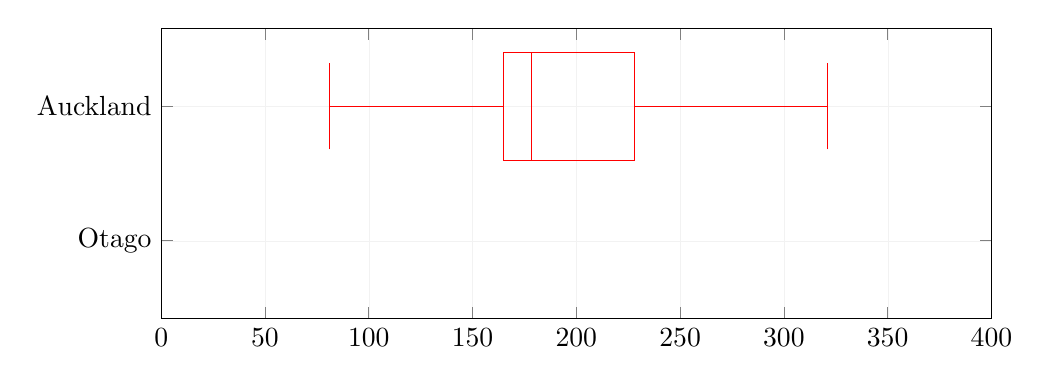
\begin{tikzpicture}
  \begin{axis}
    [
    width=\linewidth,
    height=15em,
    ytick={2,1},
    yticklabels={Auckland, Otago},
    xmin = 0, xmax = 400, xtick distance = 50,
    major grid style={line width=.1pt, draw=gray!10},
    grid = both
    ]
    \addplot[
    boxplot prepared={
      median=0,
      upper quartile=0,
      lower quartile=0,
      upper whisker=0,
      lower whisker=0
    },
    ] coordinates {};
    \addplot+[
    boxplot prepared={
      median=178.5,
      upper quartile=165,
      lower quartile=228,
      upper whisker=81,
      lower whisker=321
    },
    ] coordinates {};
  \end{axis}
\end{tikzpicture}

\clearpage
\subsection*{Questions}
\begin{questions}
  \question Fill in the University of Otago column in the table using the data given, and draw a box-and-whisker graph
            for it in the space underneath the University of Auckland graph.
  \question Write a couple of paragraphs comparing the two graphs (half a page at most) and discussing the pros and cons
            of university ranking surveys. You might want to discuss the questions below:
    \begin{parts}
      \part How do you think the ranking websites might have conducted their surveys (who did they talk to and/or what
            data might they have gathered)? What might the pros and cons of your predicted surveying method be?
      \part Is one university generally ranked higher than the other?
      \part Looking at the graphs, can you see any visible skew in the data?
      \part Do you think that the higher ranked university is necessarily better, or could there be some other reason for its
            high ranking --- in other words, does the ranking of the university actually reflect how `good' it is, or could
            there be some other force(s) at play here?
    \end{parts}
\end{questions}
\end{document}
